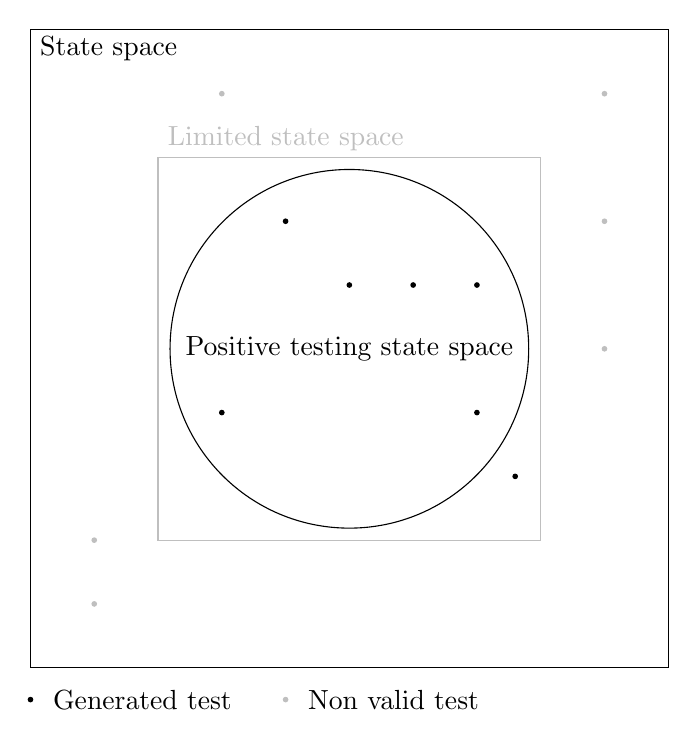
\begin{tikzpicture}[scale=0.81,
  valid/.style={fill=black},
  unvalid/.style={fill=black!25, color=black!25}]
\draw (0,0) rectangle (10,10) node [below, right] at
(0,9.7) {State space};
\draw [color=black!25] (2,2) rectangle (8,8) node [above, right] at
(2,8.3) {Limited state space};
\draw (5, 5) circle (80pt) node at (5,5) {Positive testing state space};

\draw [unvalid] (1,1) circle (1pt);
\draw [unvalid] (1,2) circle (1pt);
\draw [valid] (3,4) circle (1pt);
\draw [unvalid] (3,9) circle (1pt);
\draw [unvalid] (9,5) circle (1pt);
\draw [unvalid] (9,9) circle (1pt);
\draw [valid] (7,6) circle (1pt);
\draw [unvalid] (9,7) circle (1pt);
\draw [valid] (5,6) circle (1pt);
\draw [valid] (4,7) circle (1pt);
\draw [valid] (6,6) circle (1pt);
\draw [valid] (7,4) circle (1pt);
\draw [valid] (7.6,3) circle (1pt);

\draw [valid] (0,-0.5) circle (1pt) node [right] at (0.2,-0.5)
{Generated test};
\draw [unvalid] (4,-0.5) circle (1pt) node [right, color=black] at (4.2,-0.5)
{Non valid test};
\end{tikzpicture}